\textbf{COLUNI 2018 -- Questão 24}\par\medskip Para comparar a temperatura das mãos de Paula e das mãos de Júlia foram utilizados dois termômetros digitais. As temperaturas das mãos delas em graus Celsius, em função do tempo em segundos, são apresentadas no gráfico abaixo.

\par

% COLUNI-AUTO-FIGURES-BEGIN
\begin{figure}[htbp]
\centering
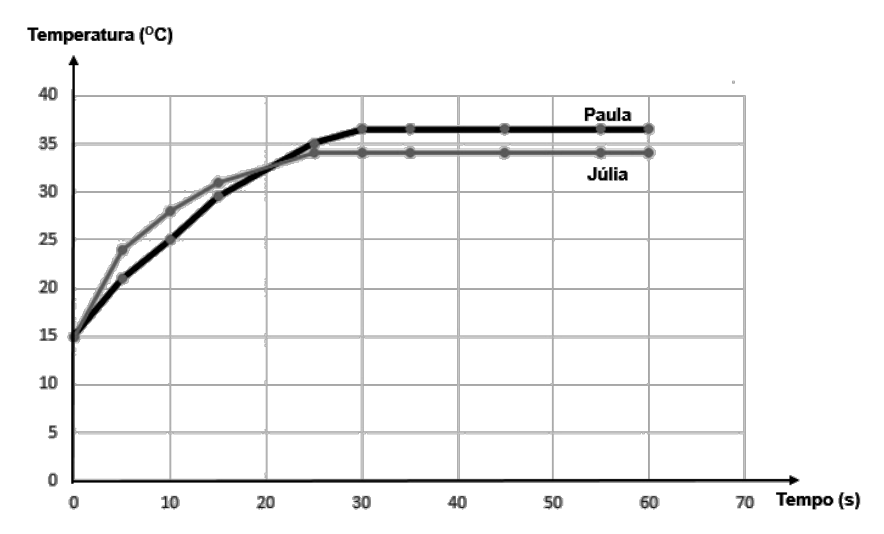
\includegraphics[width=0.95\linewidth]{static/simulados/coluni/figuras/2018/questao-24/figura-1.png}
\end{figure}
% COLUNI-AUTO-FIGURES-END

A partir do exposto no gráfico, é INCORRETO afirmar:


\begin{enumerate}
\item O termômetro em contato com a mão de Júlia atingiu a temperatura máxima mais rapidamente.
\item Em 15 s, o termômetro em contato com a mão de Júlia acusou temperatura menor.
\item Após 30 s, os termômetros estavam em equilíbrio térmico com as respectivas mãos.
\item O termômetro em contato com a mão de Paula demorou mais para entrar em equilíbrio térmico.\end{enumerate}
